% !TeX program = lualatex

\documentclass[10pt]{beamer}

\usetheme{polimi}

% Full instructions available at:
% https://github.com/elauksap/beamerthemepolimi

% Pacchetti
\usepackage{tikz}
\usetikzlibrary{positioning}
\usepackage{tabularx}
\usepackage{enumitem}
\usepackage{soul}
\usepackage[binary-units=true]{siunitx}
\usepackage{multirow}
\usepackage{array}
\usepackage{listings}
\usepackage{parcolumns}
\usepackage{graphicx}
\usepackage[font=footnotesize]{subfig}
\usepackage{mathtools}
% http://www-ljk.imag.fr/membres/Jerome.Lelong/latex/appendixnumberbeamer.sty
% Reference: http://tex.stackexchange.com/questions/2541/beamer-frame-numbering-in-appendix
\usepackage{appendixnumberbeamer}
% Add total frame count to slides, optional. From Stefan,
% http://www.latex-community.org/forum/viewtopic.php?f=4&t=2173
\expandafter\def\expandafter\insertshorttitle\expandafter{%
  \insertshorttitle\hfill\insertframenumber\,/\,\inserttotalframenumber}

% Set custom font (requires to compile with XeLaTeX).
\usepackage{ifxetex}
\ifxetex
    \usepackage{fontspec}
    \setsansfont[Scale=0.85]{Arial}
\fi

% Opzioni
%\graphicspath{{./img/}}
\pdfstringdefDisableCommands{\def\\{}}
\usetikzlibrary{arrows}
\usetikzlibrary{calc}
\setlength{\leftmargini}{10pt}
\newcommand{\norm}[1]{\left\lVert#1\right\rVert}
\newcommand{\tikzrarrow}{\tikz\draw[>=triangle 60, ->](0,0) -- (0.5,0) node{};}
\newcommand{\tikzlarrow}{\tikz\draw[>=triangle 60, <-](0,0) -- (0.5,0) node{};}
\newcommand{\tikzrarrowspace}{\tikz\draw[ ](0,0) (0.5,0) node{};}
\newcommand{\tikzlnode}[1]{\tikz[baseline=-.5ex] \node[coordinate] (#1) {};}
\newcommand{\tikzcnode}[2]{\tikz[baseline]{\node[anchor=base] (#1){#2}}}
\newcommand\Wider[2][3em]{%
    \makebox[\linewidth][c]{%
        \begin{minipage}{\dimexpr\textwidth+#1\relax}
            \raggedright#2
        \end{minipage}%
    }%
}
\tikzstyle{every picture}+=[remember picture]
\setitemize{label=\usebeamerfont*{itemize item}%
    \usebeamercolor[fg]{itemize item}
    \usebeamertemplate{itemize item}}

\title{Analysis and validation of spaceborne \\ synthetic imagery using a Vision-Based pose \\ initialization algorithm for non-cooperative \\ spacecrafts}
\subtitle{}
\author{Francescodario Cuzzocrea}
\date{\today}

\begin{document}

% Serve per eliminare Figure o Table dalle caption
\setbeamertemplate{caption}{\raggedright\insertcaption\par}
{
  \vfuzz=90pt
  %\maketitle
}

\begin{frame}
  \maketitle
\end{frame}

\section{Introduction}
% Section page.
\begin{frame}[plain]{}
  \sectionpage
\end{frame}

\begin{frame}{Table of contents}

  \bigskip

  \tableofcontents

  \vspace{0.9cm}

  \textbf{\textsc{\large Aim of the thesis}} \tikzrarrow
  Develop a data-set of images representative of in-orbit real operative conditions and test them using a Computer Vision (CV) algorithm.

\end{frame}

\begin{frame}{Motivation}

  \textsc{\textbf{\large Nowadays, different classes of missions envision a major role for close-range proximity operations}}

  \bigskip

  \begin{minipage}[t]{0.4\textwidth}
    \vspace{0.01mm}
    Purposes:
  \end{minipage}%
  \begin{minipage}[t]{0.6\textwidth}
    \vspace{0.01mm}
    \begin{itemize}[label=$\bullet$]
      \item Formation Flying (FF);
      \item On-Orbit Servicing (OOS);
      \item Active Debris Removal (ADR).
    \end{itemize}
  \end{minipage}

  \bigskip

The main challenge when performing close-range operations in OOS and ADR missions is when the target S/C may be \alert{uncooperative} (no markers or other specific supportive means). Thus, when operating in close-proximity the time evolution of the target's \alert{pose} must be estimated in autonomy by exploiting the sensors available on the S/C actively performing the servicing maneuvers.

\end{frame}

\begin{frame}{Monocular Based Pose Estimation}

  \bigskip

  \textsc{\textbf{\large Monocular Solution}}

  \bigskip

  \begin{overlayarea}{\textwidth}{0.8\textheight}
    \begin{minipage}{0.53\textwidth}
      \textbf{{Requirements}}
      \bigskip
      \hspace{1.0cm}
      \begin{itemize}[leftmargin=0.55cm]
        \item\textsc{Target 3D model availability}
        \smallskip
        \item\textsc{On-Board real-time execution}
        \smallskip
        \item\textsc{Robustness to illumination}
        \smallskip
        \item\textsc{Robustness to background}
        \smallskip
        \item\textsc{Robustness to variability of pose}
        \smallskip
      \end{itemize}
    \end{minipage}
    \hfill
    \begin{minipage}{0.44\textwidth}
      \vspace{-0.28cm}
      \hspace{0.6cm}
      \includegraphics[width=0.65\textwidth]{gfx/statoArtePose.eps}
    \end{minipage}   

    \bigskip
    
  \tikzrarrow Need a \alert{representative} data-set to develop complex \alert{CV} algorithms
    \hfill
  \end{overlayarea}

\end{frame}

\begin{frame}{Synthetic Image Generation: commercial solutions}

  \bigskip

  \begin{overlayarea}{\textwidth}{0.8\textheight}

  \hspace{0.6cm}  
  \textsc{\ul{ESA PANGU}}

  \begin{columns}[T,onlytextwidth]
    \hspace{0.6cm}
    \begin{column}{0.5\textwidth}
    \includegraphics[width=0.45\textwidth]{gfx/pangu3.eps}
    \end{column}
    \hspace{-1.5cm}
    \begin{column}{0.5\textwidth}

    \smallskip
    
    Need to be ESA project contractor    

    \smallskip
    
    \begin{itemize}[label=$\bullet$]
      \item OpenGL image rendering
      \item Can make use of GPU cores
      \item Closed-Source
    \end{itemize}
    \end{column}
  \end{columns}

  \smallskip

  \hspace{0.6cm}  
  \textsc{\ul{Airbus SurRender}}

  \begin{columns}[T,onlytextwidth]
  \hspace{0.6cm}  
    \begin{column}{0.5\textwidth}
         \includegraphics[width=0.44\textwidth]{gfx/surrender.eps}
    \end{column}
    \hspace{-1.5cm}
    \begin{column}{0.5\textwidth}

    \smallskip
    
    Need to buy a license from Airbus
  
    \smallskip
 
    \begin{itemize}[label=$\bullet$]
      \item Ray tracing image rendering
      \item Fully parallelized
      \item Closed-Source
    \end{itemize}
    \end{column}
  \end{columns}
\end{overlayarea}
\end{frame}

\begin{frame}{Synthetic Image Generation: academical solutions}

  \bigskip

  \begin{overlayarea}{\textwidth}{0.8\textheight}
  
  \hspace{0.6cm}  
  \textsc{\ul{SPEED data-set}}

  \begin{columns}[T,onlytextwidth]
    \hspace{0.6cm}
    \begin{column}{0.5\textwidth}
    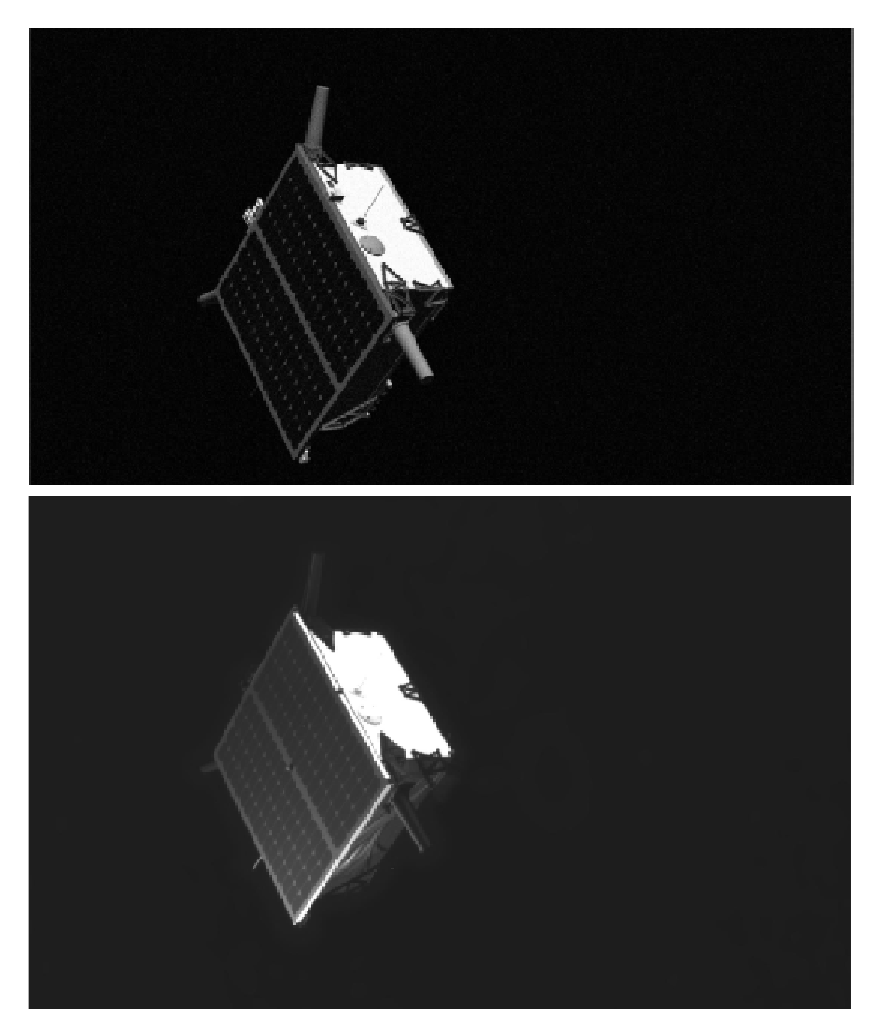
\includegraphics[width=0.4\textwidth]{gfx/speed.eps}
    \end{column}
    \hspace{-1.5cm}
    \begin{column}{0.5\textwidth}
    
    \smallskip
    
     Only the Tango S/C is represented in the images.    

    \smallskip

    \begin{itemize}[label=$\bullet$]
      \item TRON facility for real images
      \item OpenGL image rendering
      \item Closed-Source
    \end{itemize}
    \end{column}
  \end{columns}

  \smallskip

  \hspace{0.6cm}
  \textsc{\ul{URSO data-set}}

  \begin{columns}[T,onlytextwidth]
  \hspace{0.6cm}
    \begin{column}{0.5\textwidth}
        \includegraphics[width=0.58\textwidth]{gfx/URSO.eps}
    \end{column}
    \hspace{-1.5cm}
    \begin{column}{0.5\textwidth}

    \smallskip
        
    Lack of photometric accuracy    

    \smallskip
    
    \begin{itemize}[label=$\bullet$]
      \item Implemented using Unreal Engine 4
      \item Developed to train neural networks
      \item Open-Source rendering engine
    \end{itemize}
    \end{column}
  \end{columns}
\end{overlayarea}
\end{frame}

\section{Synthetic Image Generation}
% Section page.
\begin{frame}[plain]{}
  \sectionpage
\end{frame}

\begin{frame}{Introduction}
  \bigskip

  \textsc{\textbf{\large Requirements}}

  \bigskip

  \tikzrarrow Emerges the need for a tool capable of rendering images for CV algorithms \\ \tikzrarrowspace training which must:
  \smallskip
  \begin{itemize}[leftmargin=1.5cm,label=-]
    \item be affordable for small research center or small companies
    \item be capable of rendering different kinds S/C
    \item be able to accomodate solar-system sized scenes
    \item be able to also render composite background
  \end{itemize}
  \smallskip
  \tikzrarrow The images have to be \alert{representative} of a real data-set taken by a true \\ \tikzrarrowspace camera! \\
  \smallskip
  \tikzrarrow A lack of realism can lead to \alert{wrong} assumptions and thus \alert{incoherent} \\ \tikzrarrowspace results!!!

\end{frame}

\begin{frame}{Introduction}

  \bigskip

  \textsc{\textbf{\large Ray Tracing}}

  \bigskip

  \textsc{\textbf{POV-Ray represents a viable solution}}

  \smallskip

  \begin{minipage}[t]{0.5\textwidth}
    \vspace{0.01mm}
    \begin{itemize}[leftmargin=0.7cm,label=$\bullet$]
      \item Support \textbf{mesh} and objects
      \item Customizable optical properties
      \item Customizable light properties
      \item Customizable textures support
      \item Customizable camera parameters
      \item Used by ESA before PANGU
    \end{itemize}

  \end{minipage}%
  \begin{minipage}[t]{0.5\textwidth}
    \vspace{0.15cm}
    \hspace{-0.5cm}
    \centering
    \includegraphics[width=0.85\textwidth]{gfx/ray-tracing.eps}
  \end{minipage}

  \smallskip

  \tikzrarrow It simulates the physics of light! \\

  \smallskip

  \tikzrarrow Noise can be modeled and added \textit{a posteriori} to enhance fidelity. \\

  \bigskip

\end{frame}


\begin{frame}{Environment Modeling}

  \bigskip

  \textsc{\textbf{\large Earth Modeling}}

  \bigskip

  \tikzrarrow Use three different layers to differentiate optical parameters and textures \\ \tikzrarrowspace for seasonality variations

  \vspace{-0.3cm}
  \begin{columns}[T,onlytextwidth]
    \begin{column}{0.5\textwidth}
  \begin{figure}
    \captionsetup[subfigure]{labelformat=empty}
    \centering
    \subfloat[Terrain]{\includegraphics[width=0.32\textwidth]{gfx/earthMercator.eps}}
    \qquad
    \subfloat[Landmask]{\includegraphics[width=0.32\textwidth]{gfx/landmask_mercator.eps}}
    \qquad
    \subfloat[Clouds]{\includegraphics[width=0.32\textwidth]{gfx/clouds.eps}}
    \qquad
  \end{figure}
    \end{column}
    \begin{column}{0.5\textwidth}    
    \begin{figure}
    \captionsetup[subfigure]{labelformat=empty}
    \centering
    \subfloat[Same optical parameters]{\includegraphics[width=0.34\textwidth]{gfx/TerraNoAcquaNoAtmo.eps}}
    \hspace{0.5cm}
    \subfloat[Different optical paramters]{\includegraphics[width=0.34\textwidth]{gfx/TerraSiAcquaNoAtmo.eps}}
    \qquad
  \end{figure}  
    \end{column}    
    \end{columns}
  \bigskip
  \tikzrarrow The Sun has been modeled using POV-Ray \textbf{area\_light} feature
%\tikzrarrow Lack of atmospheric model
\end{frame}

%\begin{frame}{Environment Modeling}
%
%  \bigskip
%
%  \textsc{\textbf{\large Earth Modeling}}
%
%  \bigskip
%
%  \tikzrarrow Use three different layers to differentiate optical parameters and textures \\ \tikzrarrowspace for seasonality variations.
%
%  \vspace{-0.3cm}
%
%  \begin{figure}
%    \captionsetup[subfigure]{labelformat=empty}
%    \centering
%    \subfloat[True Color mercator image]{\includegraphics[width=0.32\textwidth]{gfx/earthMercator.eps}}
%    \qquad
%    \subfloat[Landmask mercator image]{\includegraphics[width=0.32\textwidth]{gfx/landmask_mercator.eps}}
%    \qquad
%    \subfloat[Cloud layer mercator image]{\includegraphics[width=0.32\textwidth]{gfx/clouds.eps}}
%    \qquad
%  \end{figure}
%
%  \bigskip

%\end{frame}

%\begin{frame}{Environment Modeling}
%
%  \bigskip
%
%  \textsc{\textbf{\large Earth Modeling}}
%
%  \bigskip
%
%  \vspace{-0.3cm}
%
%  \begin{figure}
%    \captionsetup[subfigure]{labelformat=empty}
%    \centering
%    \subfloat[No differentiation of optical parameters]{\includegraphics[width=0.34\textwidth]{gfx/TerraNoAcquaNoAtmo.eps}}
%    \hspace{0.5cm}
%    \subfloat[Differentiation of optical paramters]{\includegraphics[width=0.34\textwidth]{gfx/TerraSiAcquaNoAtmo.eps}}
%    \qquad
%  \end{figure}
%
%  \bigskip
%
%  \tikzrarrow Lack of atmosphere model.
%
%  \bigskip
%
%\end{frame}

\begin{frame}{Environment Modeling}

  \bigskip

  \textsc{\textbf{\large Earth Modeling}}

  \bigskip

  \tikzrarrow Add 25 km thick atmosphere augment realness and challenge edge \\ \tikzrarrowspace detection CV algorithms

  \vspace{-0.3cm}

  \begin{figure}
    \captionsetup[subfigure]{labelformat=empty}
    \centering
    \subfloat[No atmosphere]{\includegraphics[width=0.34\textwidth]{gfx/TerraSiAcquaNoAtmo.eps}}
    \hspace{0.5cm}
    \subfloat[Atmosphere]{\includegraphics[width=0.34\textwidth]{gfx/TerraSiAcquaSiAtmo.eps}}
    \qquad
  \end{figure}

  \bigskip

\end{frame}

\begin{frame}{Environment Modeling}

  \bigskip

  \textsc{\textbf{\large Earth Modeling}}

  \bigskip

  \tikzrarrow Binary image Comparison

  \begin{figure}
    \captionsetup[subfigure]{labelformat=empty}
    \centering
    \subfloat[]{\includegraphics[width=0.18\textwidth]{gfx/TerraNoAcquaNoAtmo.eps}}
    \hspace{0.3cm}
    \subfloat[]{\includegraphics[width=0.18\textwidth]{gfx/TerraSiAcquaNoAtmo.eps}}
    \hspace{0.3cm}
    \subfloat[]{\includegraphics[width=0.18\textwidth]{gfx/TerraSiAcquaSiAtmo.eps}}\\
    \vspace{-0.4cm}
    \subfloat[]{\includegraphics[width=0.18\textwidth]{gfx/BW_TerraNoAcquaNoAtmo.eps}}
    \hspace{0.3cm}
    \subfloat[]{\includegraphics[width=0.18\textwidth]{gfx/BW_TerraSiAcquaNoAtmo.eps}}
    \hspace{0.3cm}
    \subfloat[]{\includegraphics[width=0.18\textwidth]{gfx/BW_TerraSiAcquaSiAtmo.eps}}
  \end{figure}

  \bigskip

\end{frame}

\begin{frame}{Spacecraft Modeling}

  \bigskip

  \textsc{\textbf{\large 3D Model of the Spacecraft}}

  \bigskip

  \tikzrarrow Based on  the TANGO spacecraft from the PRISMA mission:

  \vspace{-0.38cm}
  \begin{columns}[T,onlytextwidth]
    \begin{column}{0.5\textwidth}
  \begin{figure}
    \captionsetup[subfigure]{labelformat=empty}
    \centering
    \subfloat[CAD]{\includegraphics[width=0.32\textwidth]{gfx/tangoScreenshot2.eps}}
    \qquad
    \subfloat[Blender]{\includegraphics[width=0.32\textwidth]{gfx/tangoBlenderCut.eps}}
    \qquad
    \subfloat[POV-Ray]{\includegraphics[width=0.32\textwidth]{gfx/tango_2Cut.eps}}
    \qquad
  \end{figure}
    \end{column}
    \begin{column}{0.5\textwidth}
            \vspace{0.6cm} 
    \begin{itemize}[label=$\bullet$]
      \item CAD is created using Autodesk Inventor
      \item Imported in Blender to exploit POV-Ray add-on
      \item Textures are applied
      \item Optical parameters are defined
      \item SDL code is refactord for MATLAB implementation
    \end{itemize} 
    \end{column}    
    \end{columns}
    
  \smallskip
  
  \tikzrarrow Process has to be carried out only one time

\end{frame}

\begin{frame}{Camera Modeling}

  \bigskip

  \textsc{\textbf{\large Simulate a real camera}}

  \bigskip

  \tikzrarrow POV-Ray allows to set camera aperture angle:

  \bigskip

  \begin{minipage}[t]{0.5\textwidth}

    \begin{equation*}
      A. R. = \frac{N_u}{N_v} \,
    \end{equation*}

    \begin{equation*}
      CCD_{size} = d_u \cdot N_u \,
    \end{equation*}

    \begin{equation*}
      \alpha = 2 \cdot \arctan{\left( \frac{CCD_{size}}{2 \cdot f_x} \right)} \,
    \end{equation*}
  \end{minipage}%
  \begin{minipage}[t]{0.5\textwidth}
    \vspace{0.2cm}
    \hspace{-0.9cm}
    \centering
    \begin{tabular}{cc}
      $N_u$ & Number of horizontal pixels \\
      $N_v$ & Number of vertical pixels   \\
      $f_x$ & Horizontal focal length     \\
      $f_y$ & Vertical focal length       \\
      $d_u$ & Horizontal pixel length     \\
      $d_v$ & Vertical pixel length       \\
    \end{tabular}
  \end{minipage}

  \bigskip

  \tikzrarrow Under the assumption of square CCD sensor having square pixels.

\end{frame}

\begin{frame}{Camera Modeling}

  \bigskip

  \textsc{\textbf{\large Reference Frames and Ground Truth Pose}}

  \bigskip

  \tikzrarrow POV-Ray by default works using a Left Handed Coordinate System

  \bigskip

  \hspace{0.3cm}$\bullet$ Flip it to use a Right Handed Coordinate System

  \smallskip

  \hspace{0.3cm}$\bullet$  Compute camera attitude by the knowledge of camera position \\ \hspace{0.5cm} and camera looking direction

  \smallskip

  \hspace{0.3cm}$\bullet$  Compute ground truth pose by knowledge of camera attitude \\ \hspace{0.5cm} and target attitude

  \smallskip

  \begin{minipage}[t]{1.0\textwidth}
    \begin{figure}
      \centering
      \captionsetup[subfigure]{labelformat=empty}
      \subfloat[]{\includegraphics[width=0.22\textwidth]{gfx/tangoAxesNormal.eps}}
      \hspace{0.1cm}
      \subfloat[]{\includegraphics[width=0.22\textwidth]{gfx/tangoAxesAfterRight.eps}}
      \hspace{0.1cm}
      \subfloat[]{\includegraphics[width=0.22\textwidth]{gfx/tangoAxesSky.eps}}
    \end{figure}
  \end{minipage}%

\end{frame}


\begin{frame}{Noise Modeling}

  \bigskip

  \textsc{\textbf{\large Add Gaussian withe noise and speckle noise}}

  \bigskip

  \tikzrarrow To enhance the fidelity noise is added to the image

  \begin{figure}
    \captionsetup[subfigure]{labelformat=empty}
    \centering
    \subfloat[]{\includegraphics[width=0.27\textwidth]{gfx/detailNoNoise.eps}}
    \qquad
    \subfloat[]{\includegraphics[width=0.27\textwidth]{gfx/detailNoise.eps}}
    \qquad
  \end{figure}

  Speckle: $\sigma^2 = 0.004$ \\
  Gaussian: $\sigma^2 = 0.003$

  \bigskip
\end{frame}

\begin{frame}{MATLAB Integration}

  \bigskip

  \textsc{\textbf{\large Simulink Model }}

  \bigskip

  \hspace{0.3cm}\tikzrarrow Simulate uncontrolled behavior on LEO orbit

  \smallskip

  \hspace{0.3cm}\tikzrarrow Easily extendable to include controlled behavior too

  \smallskip

  \hspace{0.3cm}\tikzrarrow Chaser constrained to be between 3 to 18 meters far from the target

  \smallskip

  \hspace{0.3cm}\tikzrarrow Extendable to simulate precise chaser approach

  \bigskip

  \textsc{\textbf{\large MATLAB Functions}}

  \bigskip

  \hspace{0.3cm}\tikzrarrow Write \texttt{.pov} SDL files for each image

  \smallskip

  \hspace{0.3cm}\tikzrarrow Annotate ground truth pose for each image

  \smallskip

  \hspace{0.3cm}\tikzrarrow Sets relevant POV-Ray options and run it

  \smallskip

  \hspace{0.3cm}\tikzrarrow Can re-parse ground truth pose for each image

  \bigskip

\end{frame}


\begin{frame}{Results}

  \bigskip

  \textsc{\textbf{\large Samples}}

  \vspace{-0.2cm}

  \begin{figure}
    \centering
    \captionsetup[subfigure]{labelformat=empty}
    \subfloat[]{\includegraphics[width=0.3\textwidth]{gfx/tango/tango_14.eps}}
    \hspace{0.2cm}
    \subfloat[]{\includegraphics[width=0.3\textwidth]{gfx/tango/tango_15.eps}}
    \hspace{0.2cm}
    \subfloat[]{\includegraphics[width=0.3\textwidth]{gfx/tango/tango_31.eps}}\\
    \vspace{-0.45cm}
    \subfloat[]{\includegraphics[width=0.3\textwidth]{gfx/tango/tango_60.eps}}
    \hspace{0.2cm}
    \subfloat[]{\includegraphics[width=0.3\textwidth]{gfx/tango/tango_259.eps}}
    \hspace{0.2cm}
    \subfloat[]{\includegraphics[width=0.3\textwidth]{gfx/tango/tango_268.eps}}
  \end{figure}

  \vspace{-0.2cm}
  \centering
  \alert{\textbf{WARNING}}: Custom POV-Ray version needed to replicate results!

  \bigskip

\end{frame}

\section{The SVD Architecture for Pose Initialization}
% Section page.
\begin{frame}[plain]{}
  \sectionpage
\end{frame}

\begin{frame}{Introduction}

  \bigskip

  \begin{overlayarea}{\textwidth}{0.8\textheight}
    \textsc{\textbf{\large Pose estimation problem}}\\
    \bigskip
    \begin{columns}[T,onlytextwidth]
      \begin{column}{.45\textwidth}
        \hspace{0.3cm}
        \centering
        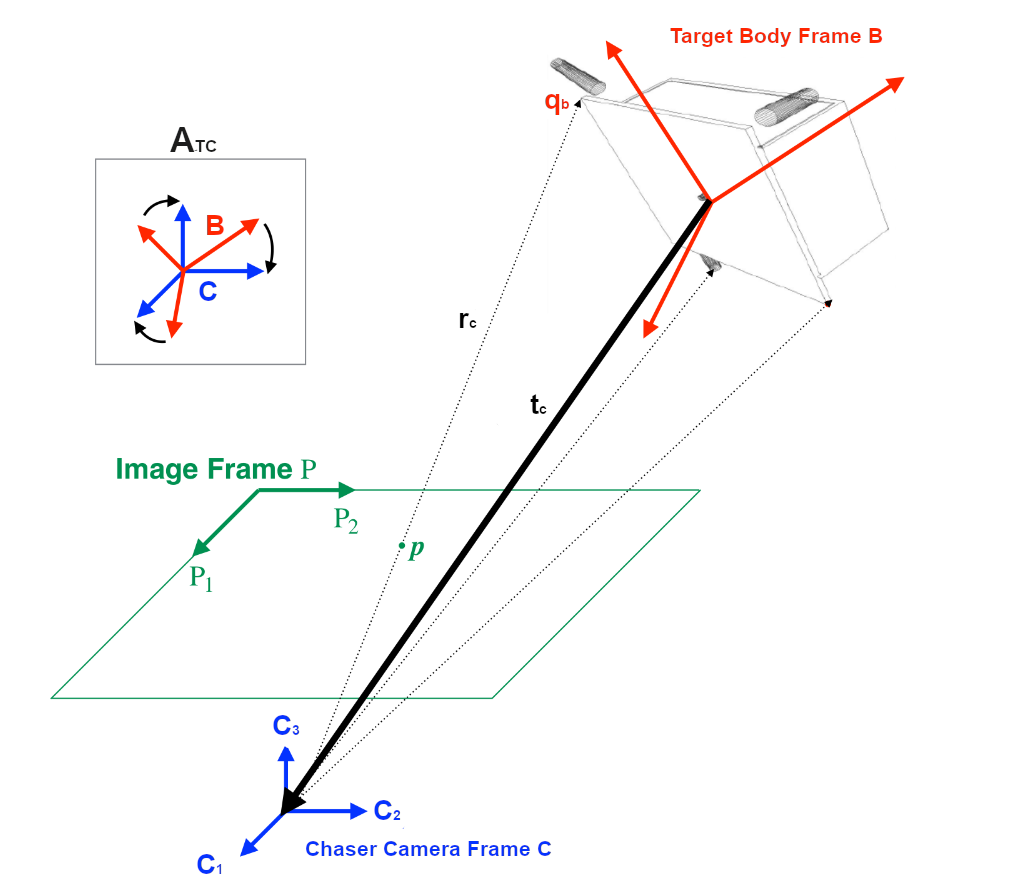
\includegraphics[width=0.8\textwidth]{gfx/poseProblem.eps}
        \smallskip
      \end{column}
      \begin{column}{.48\textwidth}
        \hspace{-0.5cm}
        \centering
        \textul{2D/3D true perspective equations}
        \vspace{0.2cm}
        \begin{equation*}
          \mathbf{r_C} = \left[x_C \quad  y_C \quad z_C\right]^T = \mathbf{A_{TC}} \; \mathbf{q_B} + \mathbf{t_C} \,
        \end{equation*}
        \vspace{-0.3cm}
        \begin{equation*}
          \mathbf{p} = \left[ \frac{x_C}{z_C} f_x + C_x , \ \frac{y_C}{z_C} f_y + C_y \right] \,
        \end{equation*}

        \vspace{0.2cm}

        \tikzrarrow $\left(\mathbf{A_{TC}},  \mathbf{t_C}\right) $ \tikzlarrow

      \end{column}
    \end{columns}
    \smallskip
    \begin{minipage}[t]{1.0\textwidth}
      \vspace{0.3cm}
      $\bullet$ Highly non linear and can have $\infty$ solutions if undercostrained\\
      $\bullet$ No \textit{a priori} knowledge of the correspondence between $\mathbf{q_B}$ and $\mathbf{p}$\\
      $\bullet$ Image has to be corrected for pixel's non-quadratism and lens distortion
    \end{minipage}%
  \end{overlayarea}

\end{frame}

\begin{frame}{Feature-based pose estimation}

  \vspace{0.2cm}

  \textsc{\textbf{\large General architecture}}

  \vspace{0.3cm}

  \tikzrarrow \textbf{Custom re-implementation of SVD algorithm from the ground up}

  \begin{minipage}[t]{1.0\textwidth}
    \centering
    \includegraphics[width=\textwidth]{gfx/SVDPipeline.eps}
  \end{minipage}%

  \vspace{0.3cm}

  \tikzrarrow \textbf{Enhance current State-of-the-art}

  \smallskip

  \begin{itemize}[leftmargin=1.1cm,label=$\bullet$]
    \item Introduces WGE technique which allows to distinguish S/C from background and allows to determine a ROI
          \smallskip
    \item Uses 2D/3D feature groups  to solve feature correspondence \\ problem
  \end{itemize}

\end{frame}

\begin{frame}{Feature-based pose estimation}

  \bigskip

  \textsc{\textbf{\large Image processing subsystem - 1}}

  \smallskip

  \begin{columns}[T,onlytextwidth]
    \hspace{-0.2cm}
    \begin{column}{0.5\textwidth}
      \includegraphics[height=0.4\textheight]{gfx/imageProcessingSubsystem.eps}
    \end{column}
    \hspace{1.2cm}
    \begin{column}{0.43\textwidth}
      \vspace{-0.2cm}
      {\small\begin{itemize}[label=$\rightarrow$]
          \item Two streams of features are extracted using Hough transform:
                {\footnotesize\begin{itemize}[topsep=0pt,label=-]
                  \item WGE stream
                  \item S\&H stream
                \end{itemize}}
          \item Multiple truncated edges are merged into one line
          \item Features are organized in perceptual groups
        \end{itemize}}
    \end{column}
  \end{columns}

  \begin{columns}[T,onlytextwidth]
    \begin{column}{0.6\textwidth}
      \begin{itemize}[leftmargin=0.45cm,label=$\bullet$]
        \item The knowledge of the ROI allows to tune Hough hyperparameters adaptively to obtain desired behavior
              \smallskip
        \item Edges outside the ROI are rejected
      \end{itemize}
    \end{column}
    \begin{column}{0.5\textwidth}
      \vspace{0.28cm}
      \centering
      \hspace{-0.95cm}
      \includegraphics[width=0.35\textwidth]{gfx/segmentsPreMerge.eps}
      \hspace{0.1cm}
      \includegraphics[width=0.35\textwidth]{gfx/segmentsAfterMerge.eps}
    \end{column}
  \end{columns}

\end{frame}

\begin{frame}{Feature-based pose estimation}

  \bigskip

  \textsc{\textbf{\large Image processing subsystem - 2}}

  \bigskip

  \tikzrarrow \textbf{Weak Gradient Eliminator}

  \smallskip

  \tikzrarrowspace Most of the gradient intensities are weak and corresponds to the feature in\\ \tikzrarrowspace the background or on the spacecraft surface.
  \vspace{-0.5cm}
  \begin{columns}[T,onlytextwidth]
    \hspace{0.2cm}
    \begin{column}{0.5\textwidth}
      \begin{figure}
        \captionsetup[subfigure]{labelformat=empty}
        \subfloat[Original image]{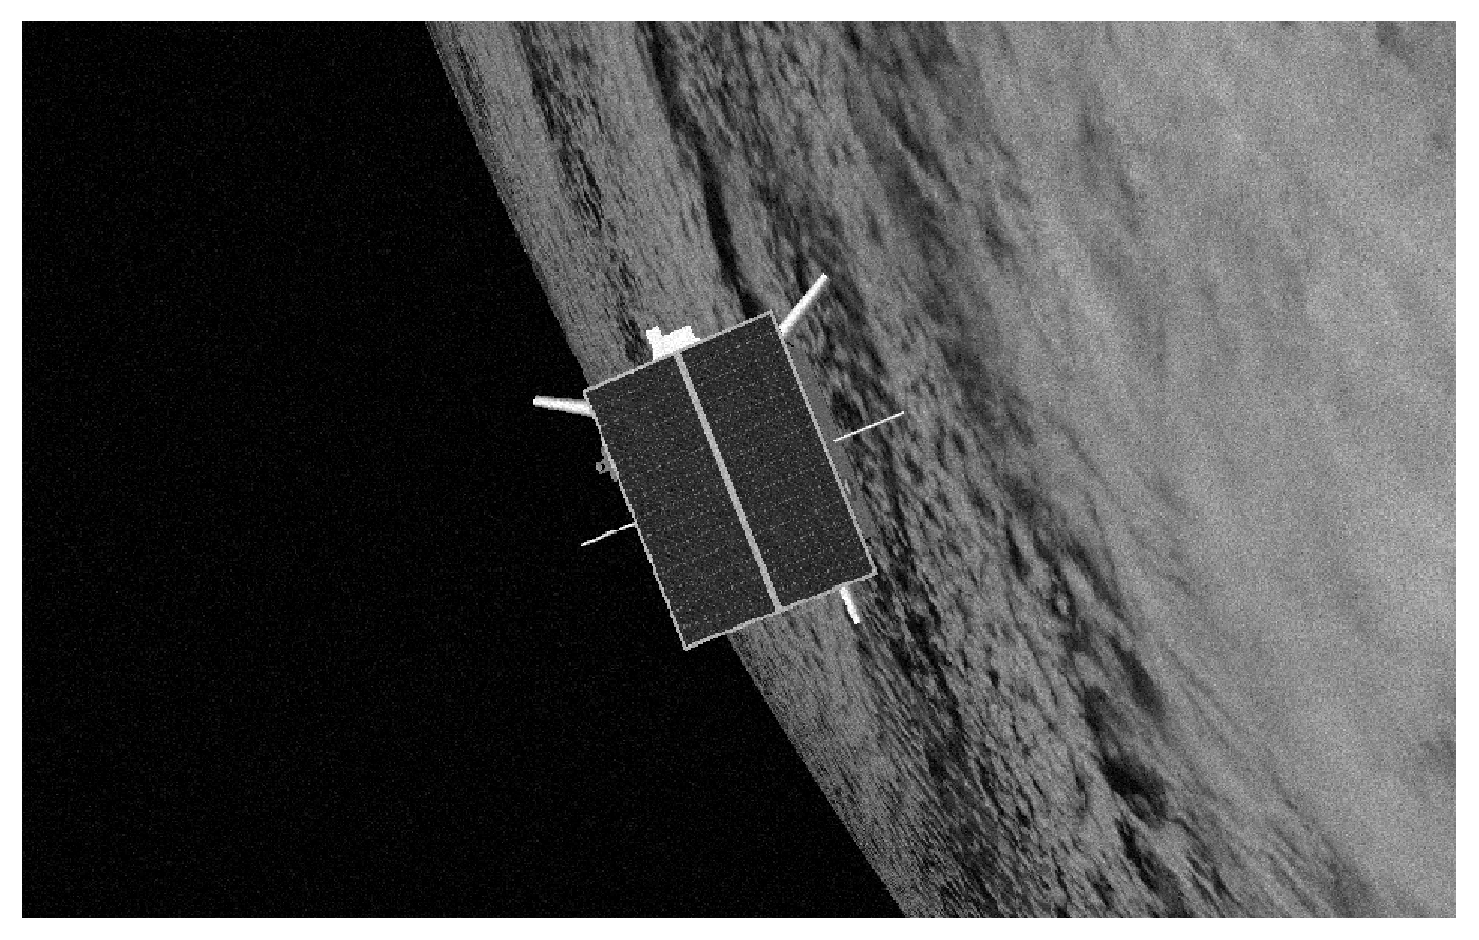
\includegraphics[width=0.41\textwidth]{gfx/FeatureDetection/chosenImage.eps}}
        \hspace{0.1cm}\subfloat[Image gradient]{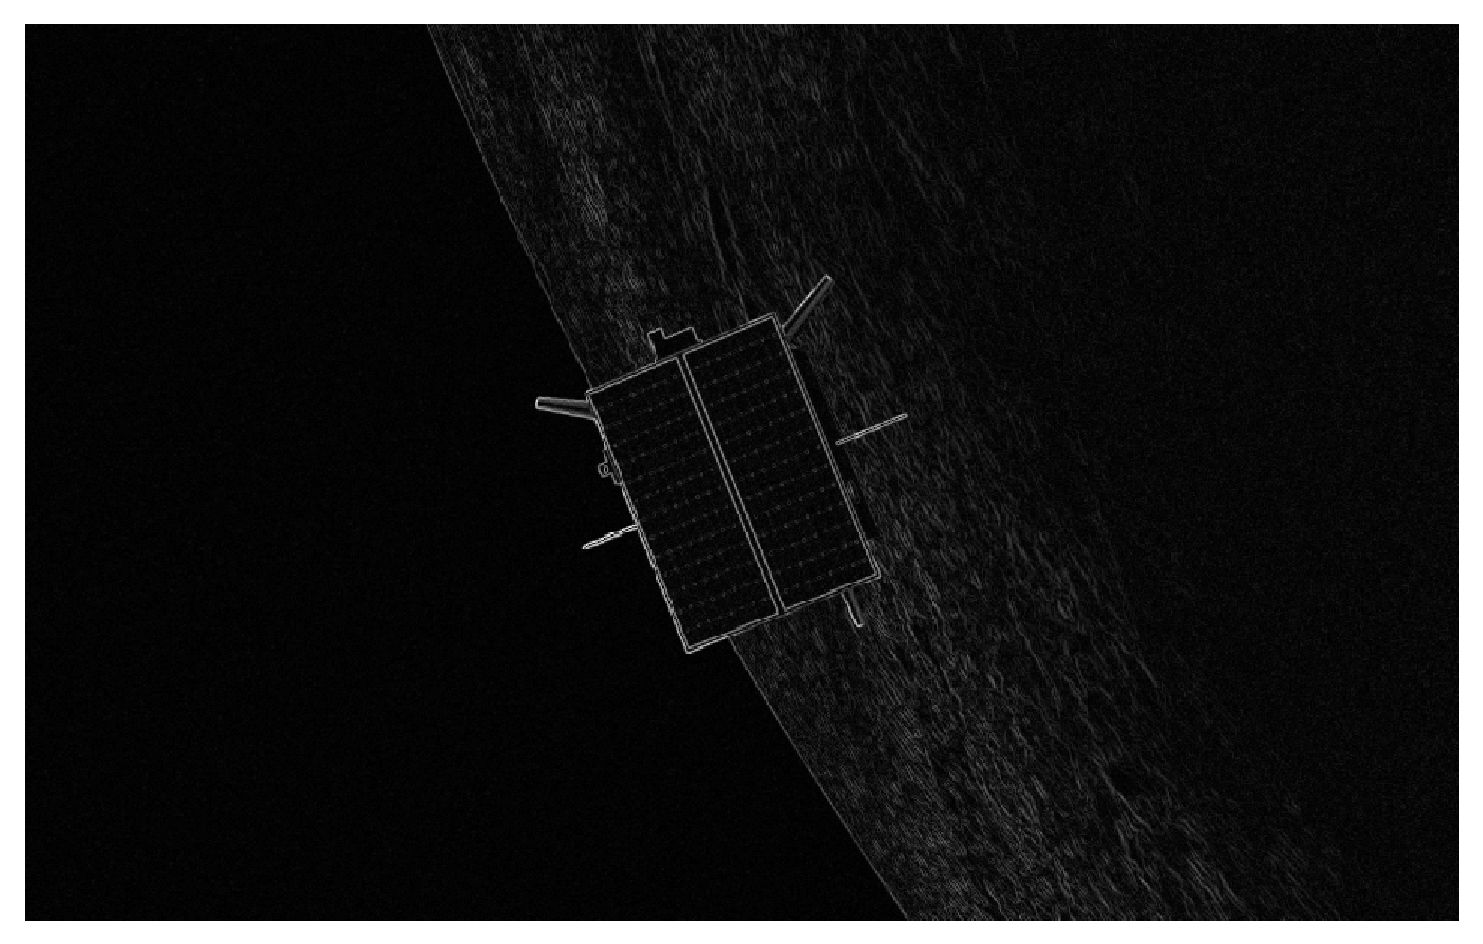
\includegraphics[width=0.41\textwidth]{gfx/FeatureDetection/gradientBeforeTresholding.eps}}\\
        \subfloat[Histogram]{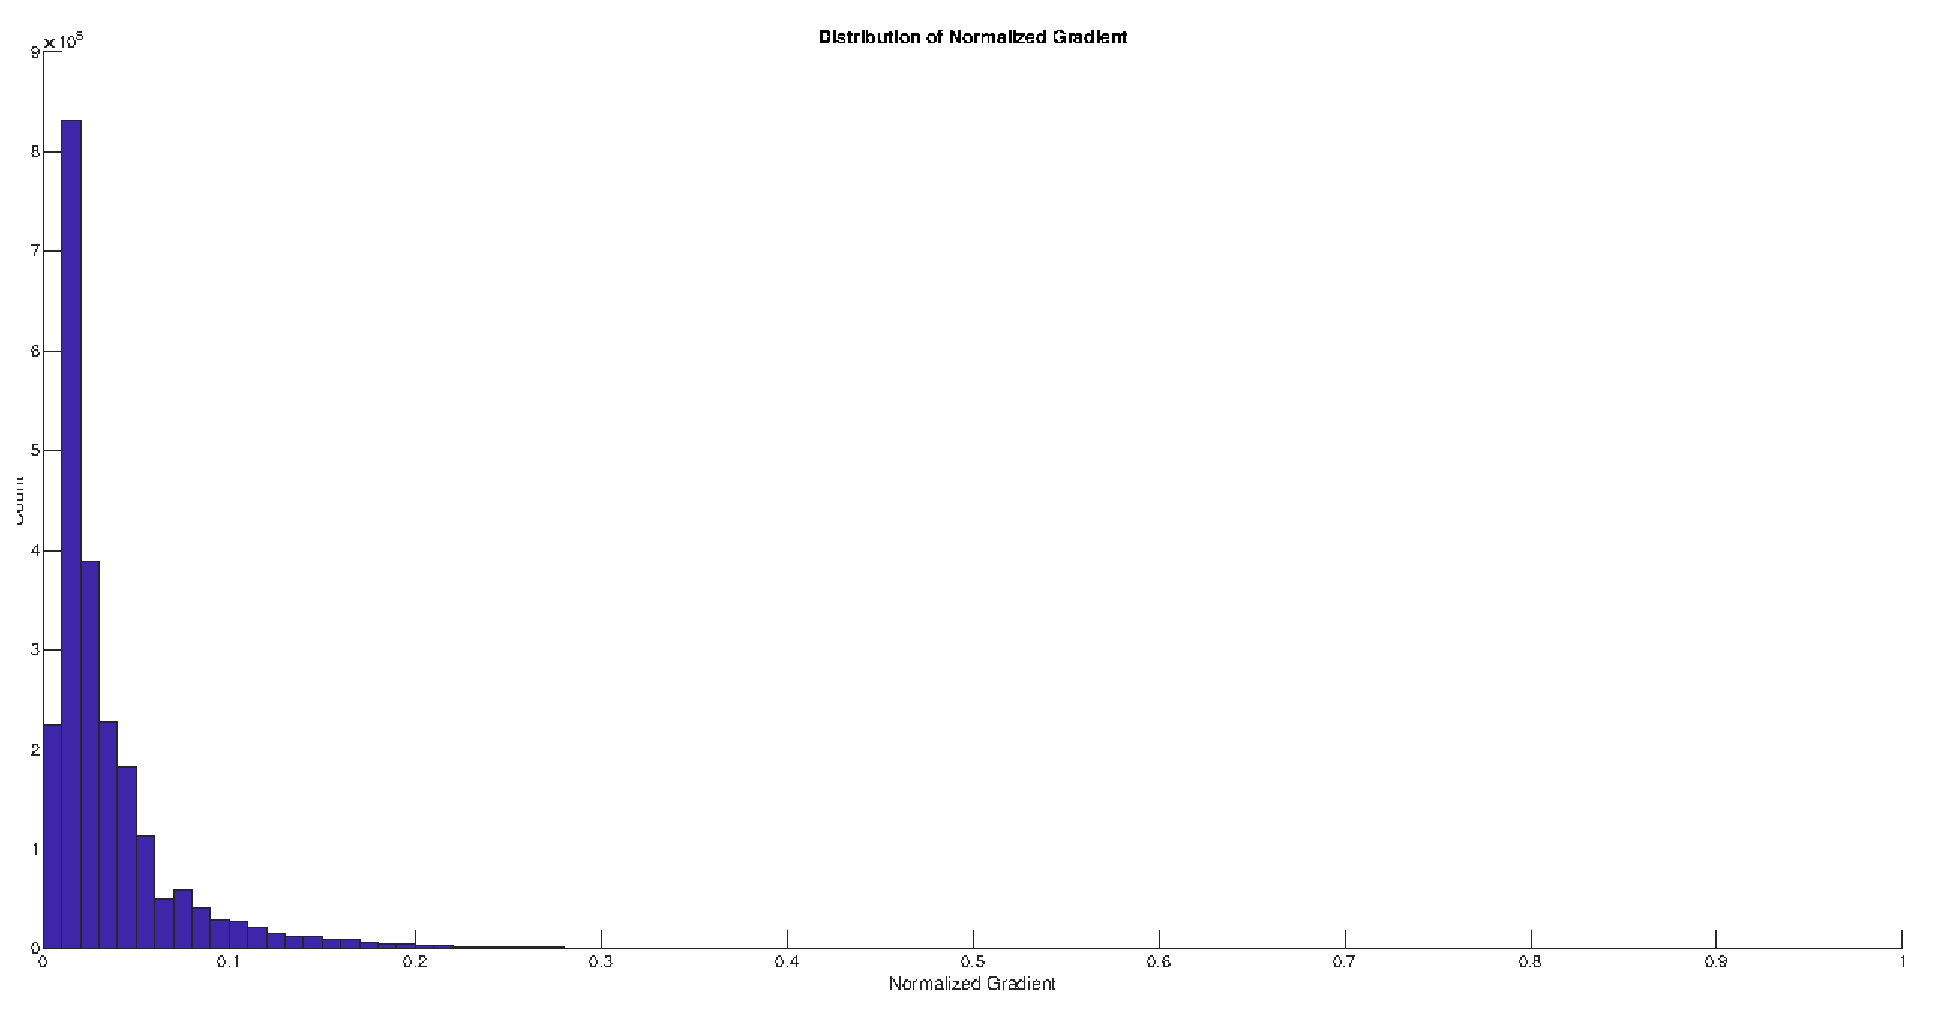
\includegraphics[width=0.41\textwidth]{gfx/FeatureDetection/gradientDistribution.eps}}
        \hspace{0.1cm}\subfloat[Filtered image]{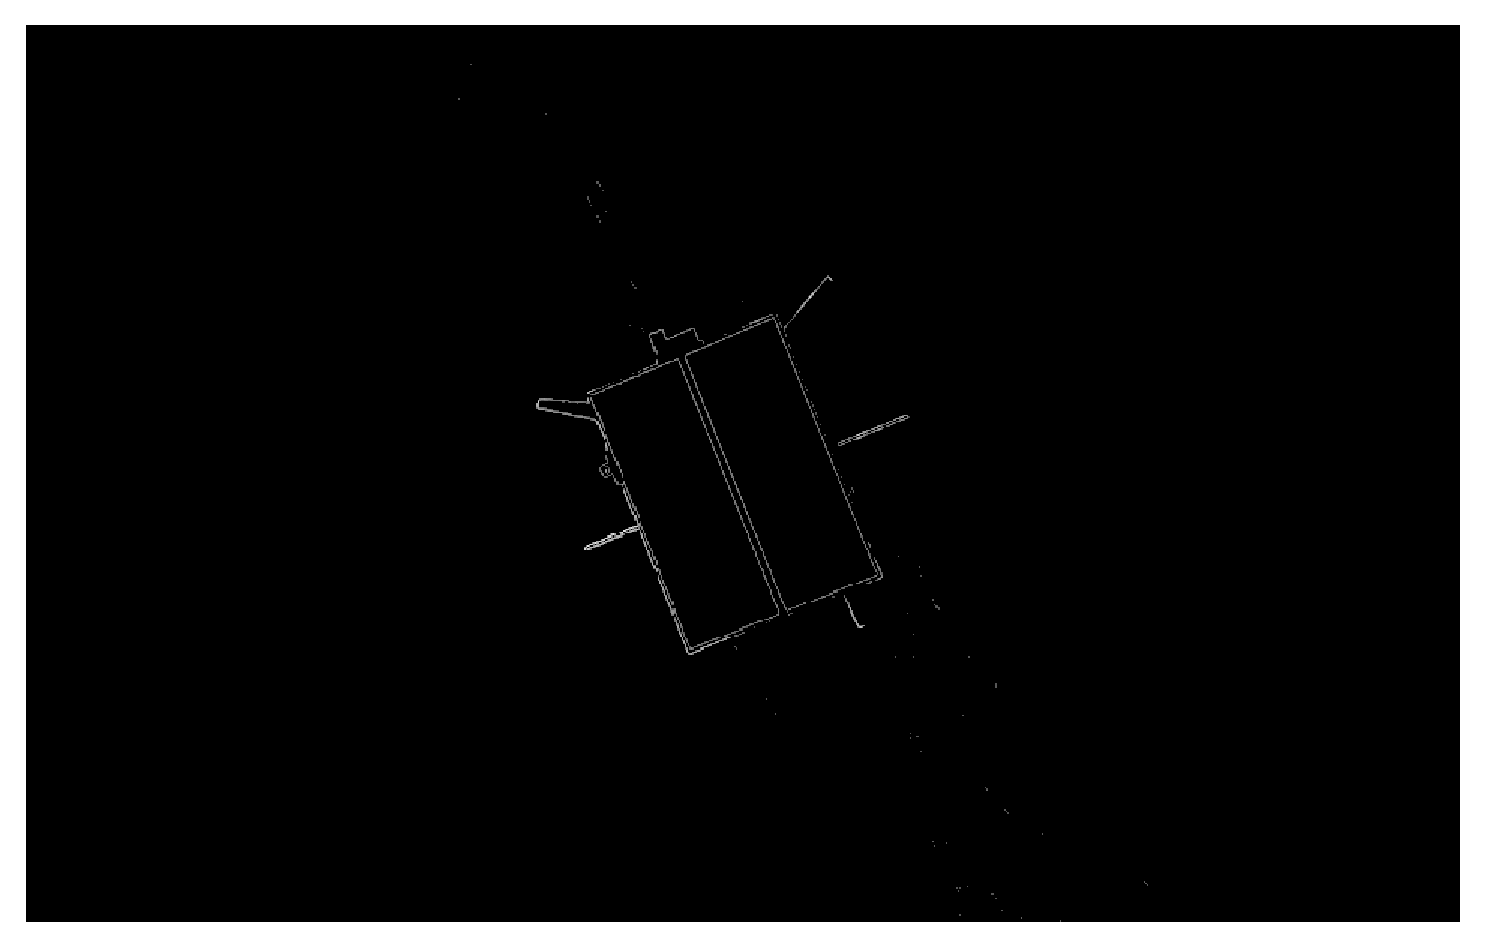
\includegraphics[width=0.41\textwidth]{gfx/FeatureDetection/imageAfterTresholding.eps}}
      \end{figure}
    \end{column}
    \begin{column}{0.5\textwidth}
      \vspace{0.65cm}
      \begin{figure}
        \captionsetup[subfigure]{labelformat=empty}
        \includegraphics[width=0.82\textwidth]{gfx/FeatureDetection/ROI.eps}
      \end{figure}
    \end{column}
  \end{columns}

\end{frame}

\begin{frame}{Feature-based pose estimation}

  \textsc{\textbf{\large Image processing subsystem - 3}}

  \bigskip

  \textsc{\textbf{\tikzrarrow Custom implementation}}

  \smallskip

  \begin{itemize}[leftmargin=0.5cm,label=$\bullet$]
    \item ROI it's enlarged by adding the 5\% of the mean detected edge length to not penalize images presenting a black background
    \item Prior applying Hough transform to the Sobel image, to eliminate the pixel chunks belonging to smaller reflective elements from the output of Hough, all connected components (objects) that have fewer than P pixels from the input binary image are removed
    \item The edge merging procedure is applied to both streams
  \end{itemize}

\end{frame}

\begin{frame}{Feature-based pose estimation}

  \textsc{\textbf{\large Image processing subsystem - 4}}

  \begin{figure}
    \centering
    \captionsetup[subfigure]{labelformat=empty}
    \subfloat[WGE stream]{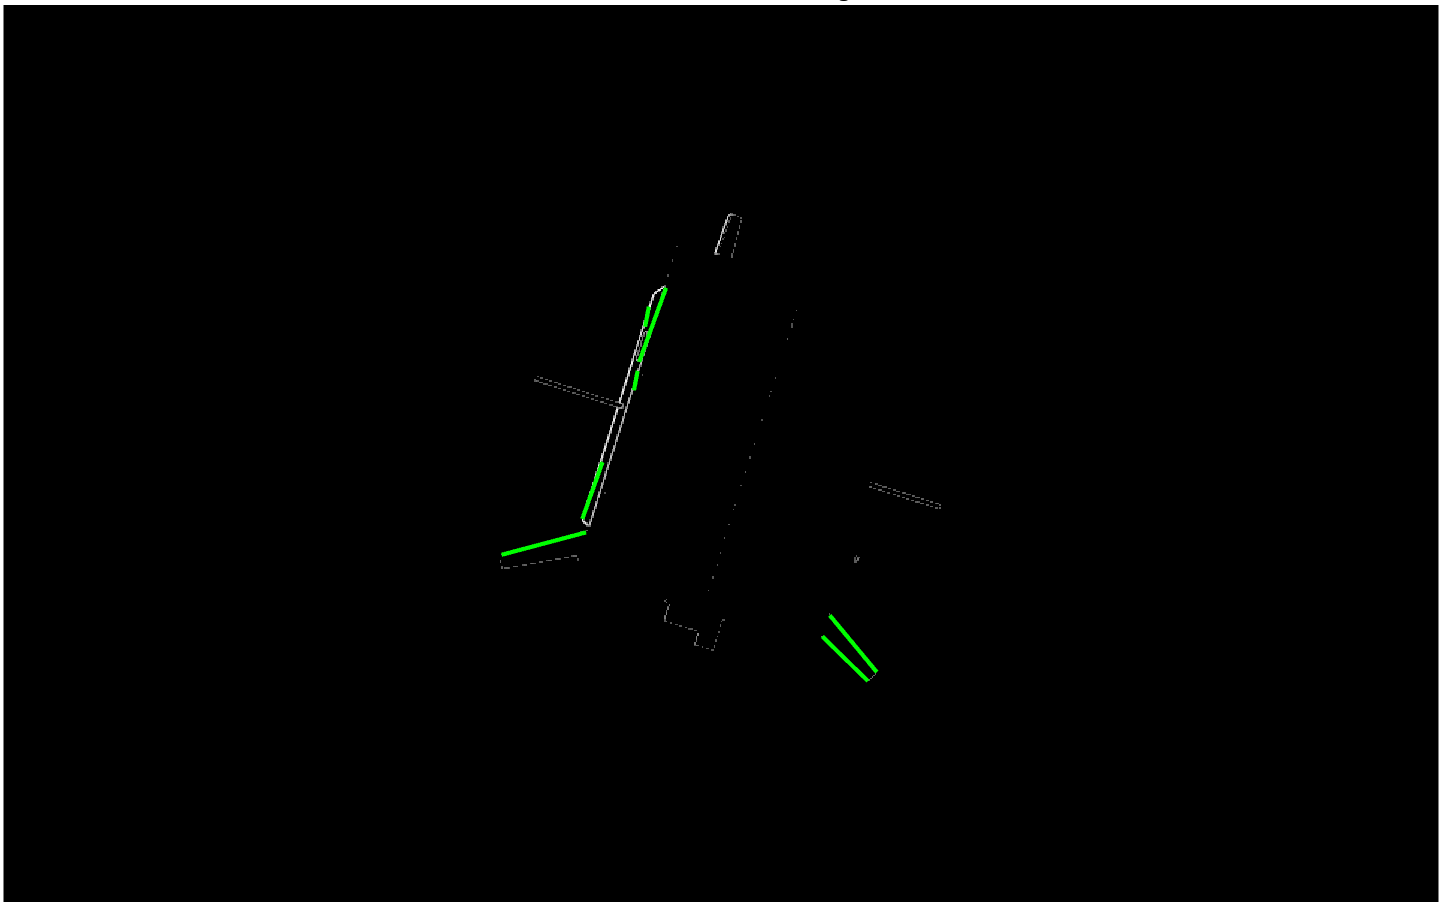
\includegraphics[width=0.25\textwidth]{gfx/FeatureDetection/214/10.png}}
    \qquad
    \subfloat[S\&H stream]{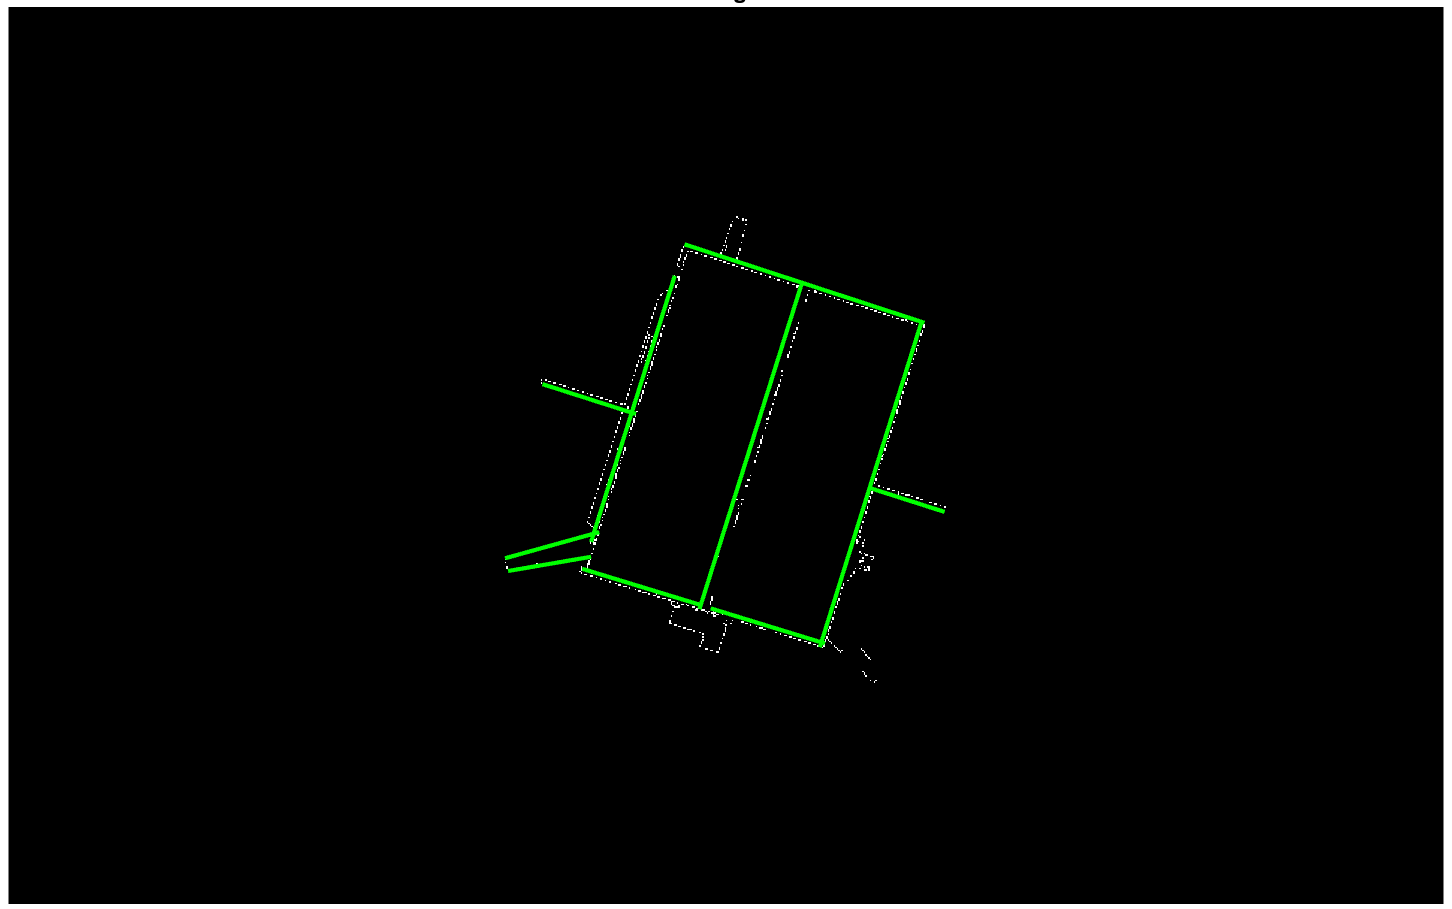
\includegraphics[width=0.25\textwidth]{gfx/FeatureDetection/214/11.png}}
    \qquad
    \subfloat[WGE merge]{\includegraphics[width=0.25\textwidth]{gfx/FeatureDetection/214/12.png}}
    \qquad
    \subfloat[S\&H merge]{\includegraphics[width=0.25\textwidth]{gfx/FeatureDetection/214/13.png}}
    \qquad
    \subfloat[WGE + S\&H]{\includegraphics[width=0.25\textwidth]{gfx/FeatureDetection/214/14.png}}
    \qquad
    \subfloat[Merge stream]{\includegraphics[width=0.25\textwidth]{gfx/FeatureDetection/214/15.png}}
  \end{figure}

\end{frame}

\begin{frame}{Feature-based pose estimation}

  \smallskip

  \textsc{\textbf{\large Perceptual Grouping}}

  \bigskip

  \textbf{\tikzrarrow Allows to reduce the search space of the correspondence problem}

  \smallskip

  \begin{columns}[T,onlytextwidth]
    \begin{column}{0.4\textwidth}
    \vspace{0.3cm}
      Perceptual groups are defined on the basis of some geometrical constraints
    \end{column}
    \begin{column}{0.5\textwidth}
      \vspace{-0.7cm}
      \begin{figure}
        \captionsetup[subfigure]{labelformat=empty}
            \hspace{-0.8cm}\subfloat[Parallel Pair]{\includegraphics[width=0.22\textwidth]{gfx/parallelPair.eps}}
        \subfloat[Proximity Pair]{\includegraphics[width=0.22\textwidth]{gfx/proximityPair.eps}}
        \subfloat[Parallel Triad]{\includegraphics[width=0.22\textwidth]{gfx/parallelTriad.eps}}
        \subfloat[Proximity Triad]{\includegraphics[width=0.22\textwidth]{gfx/proximityTriad.eps}}
        \subfloat[Closed Polygonal Tetrad]{\includegraphics[width=0.22\textwidth]{gfx/closedPolygonalTetrad.eps}}
      \end{figure}
    \end{column}
  \end{columns}

  \bigskip

  \begin{columns}[T,onlytextwidth]
    \begin{column}{0.6\textwidth}
      \vspace{0.38cm}
      \hspace{-0.3cm}
      \includegraphics[width=0.45\textwidth]{gfx/cadFull.eps}
      \hspace{0.1cm}
      \includegraphics[width=0.45\textwidth]{gfx/wireframeModel.eps}
    \end{column}
    \hspace{0.2cm}
    \begin{column}{0.45\textwidth}
    Carried out on a wireframe\\ model too by applying 3D\\ geometry definitions\\ instead of 2D ones
    \end{column}
  \end{columns}

\end{frame}

\begin{frame}{Result}

  \bigskip

  \textsc{\textbf{\large Successful pose initialization}}\\

  \bigskip

  \tikzrarrow Obtained using P3P solver coupled with a RANSAC algorithm for outlier\\ \tikzrarrowspace rejection instead of ePnP

  \vspace{-0.6cm}

  \begin{columns}[T,onlytextwidth]
    \begin{column}{0.5\textwidth}
      \begin{figure}
        \centering
        \captionsetup[subfigure]{labelformat=empty}
        \setbox1=\hbox{\includegraphics[width=0.48\textwidth]{gfx/poseDetermination/trial49modelMap.eps}}% The smaller image
        \setbox2=\hbox{\includegraphics[width=0.48\textwidth]{gfx/poseDetermination/cameraWRTSC49.eps}}% The larger image
        {\,} \hfill
        \subfloat[]{%
          \raisebox{0.5\ht2-0.5\ht1}{\includegraphics[width=0.48\textwidth]{gfx/poseDetermination/trial49modelMap.eps}}} \hfill
        \subfloat[]{%
          \includegraphics[width=0.48\textwidth]{gfx/poseDetermination/cameraWRTSC49.eps}} \hfill
        {\,}
      \end{figure}
    \end{column}

    \begin{column}{0.5\textwidth}

      \vspace{0.38cm}

      \begin{figure}
        \centering
        \captionsetup[subfigure]{labelformat=empty}
        \setbox1=\hbox{\includegraphics[width=0.48\textwidth]{gfx/poseDetermination/trial311modelMap.eps}}% The smaller image
        \setbox2=\hbox{\includegraphics[width=0.48\textwidth]{gfx/poseDetermination/cameraWRTSC311.eps}}% The larger image
        {\,} \hfill
        \subfloat[]{%
          \raisebox{0.5\ht2-0.5\ht1}{\includegraphics[width=0.45\textwidth]{gfx/poseDetermination/trial311modelMap.eps}}} \hfill
        \subfloat[]{%
          \includegraphics[width=0.48\textwidth]{gfx/poseDetermination/cameraWRTSC311.eps}} \hfill
        {\,}
      \end{figure}
    \end{column}
  \end{columns}

   \vspace{-0.2cm}

  Figures are showing the map superposed to the image and the 3D camera pose in map coordinates

\end{frame}

\section{Results}
% Section page.
\begin{frame}[plain]{}
  \sectionpage
\end{frame}

\begin{frame}{Qualitative Assessment}

  \bigskip

  \textsc{\textbf{\large SPEED VS Implemented Tool}}

  \bigskip

  \begin{minipage}[t]{1.0\textwidth}
    \begin{figure}
      \centering
      \captionsetup[subfigure]{labelformat=empty}
      \subfloat[Unfiltered Image]{\includegraphics[width=0.25\textwidth]{gfx/comparison/comp2/1.eps}}
      \qquad
      \subfloat[Histogram]{\includegraphics[width=0.3\textwidth]{gfx/comparison/comp2/3.eps}}
      \qquad
      \subfloat[Sobel Image]{\includegraphics[width=0.25\textwidth]{gfx/comparison/comp2/5.eps}}
      \qquad
      \subfloat[Unfiltered Image]{\includegraphics[width=0.25\textwidth]{gfx/comparison/comp2/2.eps}}
      \qquad
      \subfloat[Histogram]{\includegraphics[width=0.3\textwidth]{gfx/comparison/comp2/4.eps}}
      \qquad
      \subfloat[Sobel Image]{\includegraphics[width=0.25\textwidth]{gfx/comparison/comp2/6.eps}}
      \qquad
    \end{figure}
  \end{minipage}%
\end{frame}

\begin{frame}{Qualitative Assessment}

  \bigskip

  \textsc{\textbf{\large SPEED VS Implemented Tool}}

  \bigskip

  \begin{minipage}[t]{1.0\textwidth}
    \begin{figure}
      \centering
      \captionsetup[subfigure]{labelformat=empty}
      \subfloat[Unfiltered Image]{\includegraphics[width=0.25\textwidth]{gfx/comparison/comp4/1.eps}}
      \qquad
      \subfloat[Histogram]{\includegraphics[width=0.3\textwidth]{gfx/comparison/comp4/3.eps}}
      \qquad
      \subfloat[Sobel Image]{\includegraphics[width=0.25\textwidth]{gfx/comparison/comp4/5.eps}}
      \qquad
      \subfloat[Unfiltered Image]{\includegraphics[width=0.25\textwidth]{gfx/comparison/comp4/2.eps}}
      \qquad
      \subfloat[Histogram]{\includegraphics[width=0.3\textwidth]{gfx/comparison/comp4/4.eps}}
      \qquad
      \subfloat[Sobel Image]{\includegraphics[width=0.25\textwidth]{gfx/comparison/comp4/6.eps}}
      \qquad
    \end{figure}
  \end{minipage}%
\end{frame}

\begin{frame}{SVD Algorithm}

  \bigskip

  \textsc{\textbf{\large Failures}}

  \smallskip

  ROI Detection \tikzrarrow Due to composite background

  \begin{minipage}[t]{1.0\textwidth}

    \begin{figure}
      \centering
      \captionsetup[subfigure]{labelformat=empty}
      \subfloat[Detected ROI]{\includegraphics[width=0.27\textwidth]{gfx/roiFailure/1.eps}}
      \hspace{0.1cm}
      \subfloat[Normalized Gradient]{\includegraphics[width=0.27\textwidth]{gfx/roiFailure/2.eps}}\\
      \subfloat[Tresholded Gradient]{\includegraphics[width=0.27\textwidth]{gfx/roiFailure/3.eps}}
      \hspace{0.1cm}
      \subfloat[Edge Detection]{\includegraphics[width=0.27\textwidth]{gfx/roiFailure/4.eps}}
    \end{figure}
  \end{minipage}%

\end{frame}

\begin{frame}{SVD Algorithm}

  \bigskip

  \textsc{\textbf{\large Failures}}

  \smallskip

  Edge Detection \tikzrarrow Due to solar panels or distance

  \begin{minipage}[t]{1.0\textwidth}
    \begin{figure}
      \centering
      \captionsetup[subfigure]{labelformat=empty}
      \subfloat[WGE Stream]{\includegraphics[width=0.22\textwidth]{gfx/panelFailure/1.eps}}
      \hspace{0.1cm}
      \subfloat[S\&H Stream]{\includegraphics[width=0.22\textwidth]{gfx/panelFailure/2.eps}}
      \hspace{0.1cm}
      \subfloat[Merging streams]{\includegraphics[width=0.22\textwidth]{gfx/panelFailure/3.eps}}
    \end{figure}
  \end{minipage}%

  \bigskip

  \begin{minipage}[t]{1.0\textwidth}
    \begin{figure}
      \centering
      \captionsetup[subfigure]{labelformat=empty}
      \subfloat[Tresholded Gradient]{\includegraphics[width=0.22\textwidth]{gfx/distanceFailure/1.eps}}
      \hspace{0.1cm}
      \subfloat[WGE Stream]{\includegraphics[width=0.22\textwidth]{gfx/distanceFailure/2.eps}}
      \hspace{0.1cm}
      \subfloat[S\&H Stream]{\includegraphics[width=0.22\textwidth]{gfx/distanceFailure/3.eps}}
      \hspace{0.1cm}
      \subfloat[Merging Streams]{\includegraphics[width=0.22\textwidth]{gfx/distanceFailure/4.eps}}
    \end{figure}
  \end{minipage}%

\end{frame}

\begin{frame}{SVD Algorithm}

  \bigskip

  \textsc{\textbf{\large Rotational and translational errors}}

  \bigskip

  \begin{minipage}[t]{0.4\textwidth}
    \vspace{0.01mm}
    Translational Error\\

    \smallskip

    \hspace{0.3cm}\tikzrarrow Mean error: $0.2506$ m

  \end{minipage}%
  \begin{minipage}[t]{0.6\textwidth}
    \vspace{0.01mm}
    \centering
    \includegraphics[width=0.73\textwidth]{gfx/plotError/transHist.eps}
  \end{minipage}

  \smallskip

  \begin{minipage}[t]{0.4\textwidth}
    \vspace{0.01mm}
    Rotational Error\\

    \smallskip

    \hspace{0.3cm}\tikzrarrow Mean error: $0.0528^\circ$

  \end{minipage}%
  \begin{minipage}[t]{0.6\textwidth}
    \vspace{0.01mm}
    \centering
    \includegraphics[width=0.73\textwidth]{gfx/plotError/rotHist.eps}
  \end{minipage}

  \bigskip

\end{frame}

\begin{frame}{SVD Algorithm}

  \bigskip

  \textsc{\textbf{\large Errors WRT inter-spacecraft distance}}

  \bigskip

  \begin{minipage}[t]{0.4\textwidth}
    \vspace{0.01mm}
    Translational Error\\

    \smallskip

    \hspace{0.3cm}\tikzrarrow Increases with distance

  \end{minipage}%
  \begin{minipage}[t]{0.6\textwidth}
    \vspace{0.01mm}
    \centering
    \includegraphics[width=0.73\textwidth]{gfx/plotError/transAndDist.eps}
  \end{minipage}

  \smallskip

  \begin{minipage}[t]{0.4\textwidth}
    \vspace{0.01mm}
    Rotational Error\\

    \smallskip

    \hspace{0.3cm}\tikzrarrow No recognizable trend

  \end{minipage}%
  \begin{minipage}[t]{0.6\textwidth}
    \vspace{0.01mm}
    \centering
    \includegraphics[width=0.73\textwidth]{gfx/plotError/rotAndDist.eps}
  \end{minipage}

  \bigskip

\end{frame}

\begin{frame}{SVD Algorithm}

  \bigskip

  \textsc{\textbf{\large Camera axis error}}

  \bigskip

  \tikzrarrow No preferred axis

  \bigskip

  \centering
  \includegraphics[width=0.8\textwidth]{gfx/plotError/c3c2c1.eps}

  \bigskip

\end{frame}

\section{Conclusions}
% Section page.
\begin{frame}[plain]{}
  \sectionpage
\end{frame}

\begin{frame}{Results Summary}

  \bigskip

  \textsc{\textbf{\large Image Generation Tool}}

  \smallskip

  \hspace{0.3cm}\tikzrarrow Image toolbox is fully automated

  \smallskip

  \hspace{0.3cm}\tikzrarrow Controlled and uncontrolled behavior can be simulated \\ \hspace{0.3cm}\tikzrarrowspace as well as well as approach

  \smallskip

  \hspace{0.3cm}\tikzrarrow Generated images seems are promising

  \bigskip

  \textsc{\textbf{\large SVD Algorithm}}

  \smallskip

  \hspace{0.3cm}\tikzrarrow Successfully tested SVD algorithm

  \smallskip

  \hspace{0.3cm}\tikzrarrow Results seems to be promising

\end{frame}

\begin{frame}{Improvements}

  \bigskip

  \textsc{\textbf{\large Image Generation Tool}}

  \smallskip

  \hspace{0.3cm}\tikzrarrow Use better textures for the S/C and the Earth

  \smallskip

  \hspace{0.3cm}\tikzrarrow Use a more rigorous method to set optical parameters

  \smallskip

  \hspace{0.3cm}\tikzrarrow Improve noise model

  \smallskip

  \hspace{0.3cm}\tikzrarrow Patch POV-Ray code to allow GPU cores usage for rendering

  \bigskip

  \textsc{\textbf{\large SVD Algorithm}}

  \smallskip

  \hspace{0.3cm}\tikzrarrow Employ separated Hough transforms to detect different geometric\\ \hspace{0.3cm}\tikzrarrowspace shapes

  \smallskip

  \hspace{0.3cm}\tikzrarrow Improve edge detection procedure (solar panels, distance are an issue)

  \smallskip

  \hspace{0.3cm}\tikzrarrow Compare different pose solvers

  \smallskip

  \hspace{0.3cm}\tikzrarrow Hardware-in-the-loop experiments to evaluate the computational time\\ \hspace{0.3cm}\tikzrarrowspace on real H/W.

  \bigskip

\end{frame}

\begin{frame}{The End}

  \bigskip

  \centering \Large
  \emph{Thanks for your attention}
\end{frame}

\appendix
\section{Additional Material}

% Section page.
\begin{frame}[plain]{}
  \sectionpage
\end{frame}


\begin{frame}{Environment Modeling}

  \bigskip

  \textsc{\textbf{\large Light Modeling}}

  \bigskip

  \tikzrarrow The Sun can be modeled using POV-Ray \textbf{area\_light} feature:

  \smallskip

  \begin{itemize}[leftmargin=1.2cm,label=$\bullet$]
    \item it create a cluster of point-like light sources distributed on a disc
    \item the radius of the disc is set to the radius of the Sun, and placed at the exact distance which the Sun has from the Earth
    \item the \textbf{orient} option makes every object see the Sun’s disc as oriented toward it, from any position around it
  \end{itemize}

\end{frame}

\begin{frame}{Spacecraft Modeling}

  \bigskip

  \textsc{\textbf{\large 3D Model of the Spacecraft}}

  \bigskip

  \tikzrarrow Based on  the TANGO spacecraft from the PRISMA mission:

  \smallskip

 \begin{minipage}[t]{0.5\textwidth}
    \vspace{1.0cm}
    \begin{itemize}[leftmargin=0.7cm,label=$\bullet$]
      \item 570 mm x 759 mm solar panel
      \item 560 mm x 550 mm x 300 mm body
      \item 4x 204 mm antennas
    \end{itemize}
  \end{minipage}%
  \begin{minipage}[t]{0.5\textwidth}
    \vspace{0.01cm}
    \hspace{-0.2cm}
    \centering
    \includegraphics[width=0.85\textwidth]{gfx/tangoScreenshot2.eps}
  \end{minipage}

\end{frame}

\begin{frame}{Spacecraft Modeling}

  \bigskip

  \textsc{\textbf{\large 3D model rendering with POV-Ray}}

  \bigskip

  Blender POV-Ray add-on code has to be refactored to allow using one single S/C object 

  \bigskip

  \centering
  \includegraphics[width=0.5\textwidth]{gfx/tango_1.eps}

  \bigskip

\end{frame}

\begin{frame}{Spacecraft Modeling}

  \bigskip

  \textsc{\textbf{\large Bounding issue}}

  \bigskip

This system compartmentalizes all finite objects in a scene into invisible rectangular boxes that are arranged in a tree-like hierarchy. Before testing the objects within the bounding boxes the tree is descended and only those objects whose bounds are hit by a ray are tested.

  \smallskip

  \begin{figure}
    \captionsetup[subfigure]{labelformat=empty}
    \centering
    \subfloat[Bounding on]{\includegraphics[width=0.27\textwidth]{gfx/tangoNoMb.eps}}
    \qquad
    \subfloat[Bounding off]{\includegraphics[width=0.27\textwidth]{gfx/tangoMb.eps}}
    \qquad
  \end{figure}

  \bigskip
\end{frame}

\end{document}